% =========================================================
% CONFIGURACION DEL DOCUMENTO
% =========================================================
\providecommand{\main}{..}
\documentclass[../main.tex]{subfiles}

% =========================================================
% CONTENIDO
% =========================================================
\begin{document}		
\chapter{Estado del arte}
\label{cha:02_estado_del_arte}
	% ===============================================================
	% ===============================================================
	\section{Movimiento ocular}
	\label{sec:02_movimiento_ocular}
		La acción de dirigir la mirada hacia un objeto (\textit{fixation point}) es parte fundamental del proceso de visión. Este acto involucra el direccionamiento de los \gls{ejevisual} (ver figura \ref{fig:02_eye_axis}) hacia un objetivo determinado, permitiendo la realización de análisis visuales precisos. Dicha orientación muchas veces implica movimientos coordinados de los ojos, cuello y cabeza, no obstante, existen movimientos más pequeños que son realizados únicamente por los ojos, conocidos como movimientos sacádicos \cite{article:movOcular1, article:movOcular2}.
		\begin{figure}[H]
			\centering
			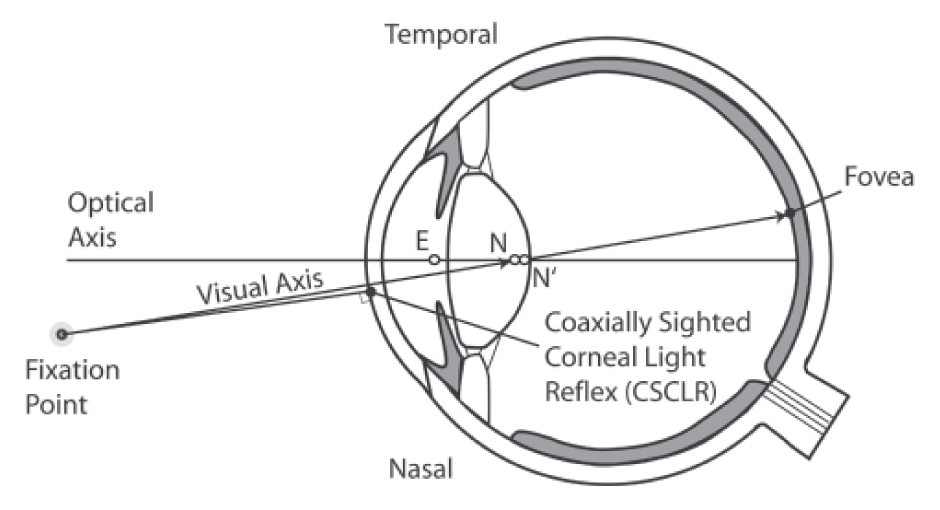
\includegraphics[width=0.45\textwidth]{cap_02_eye_axis}
			\caption[Estructura del ojo]{Estructura del ojo\footnotemark.}
			\label{fig:02_eye_axis}
		\end{figure}
		\footnotetext{Fuente imagen: J. T. Schwiegerling, ''Eye Axes and Their Relevance to Alignment of Corneal Refractive Procedures'', Journal of Refractive Surgery, vol 29(8), pp. 515-516, fig. 1-D.}

		En la figura \ref{fig:02_eye_axis} se observa un esquema simplificado del ojo observado desde la parte superior de la cabeza. En ella pueden apreciarse las proyecciones del eje óptico (\textit{optical axis}) y visual (\textit{visual axis}) del ojo, que corresponden a líneas imaginarias que van desde el centro de la retina y fóvea respectivemente, pasando por la parte posterior del cristalino y extendiéndose luego a través de la pupila y córnea.  

		Los movimientos sacádicos corresponden a las rotaciones que realiza el globo ocular entre dos momentos de posicionamiento estacionario, por tanto se traducen en el consecuente desplazamiento de la pupila. Dichos movimientos pueden ocurrir tanto en el eje horizontal como vertical y se encuentra aún en discusión \cite{article:movOcular2, article:movOcular3} si se entrega información visual en todo momento o solo es relevante al mantener la mirada detenida en alguna posición. Los movimientos sacádicos ocurren en todo momento y pueden estar provocados por procesos cognitivos conscientes o inconscientes. Independientemente de la naturaleza de estos movimientos, ambos generan patrones que permiten la construcción de un mapa mental de la escena observada. La necesidad de redireccionar el eje visual constantantemente para analizar una imagen se relaciona con la idea de que, en el ojo humano, solo la parte central de la retina (\gls{fovea}) se encuentra encargada de la visión en alta resolución, pues presenta una alta concentración de células fotorreceptoras sensibles al color. 

		Existen dos tipos de movimientos sacádicos: Los voluntarios, también conocidos como provocados, que implican control consciente sobre los procesos cognitivos y los reflexivos o automáticos, que corresponden a la respuesta natural a la aparición de un nuevo estímulo visual.

		Las características principales de dichos movimientos son:
		\begin{enumerate}\setlength\itemsep{-0.2em}
			\item Por su naturaleza los movimientos sacádicos se consideran balísticos, lo que quiere decir que la posición de destino no cambia durante el desarrollo del movimiento. Esto puede entenderse también como que el objetivo se encuentra predeterminado en el momento de partida.

			\item La velocidad de las sacadas\footnote{Forma de referirse a un movimiento sacádico.} aumenta de forma no lineal en la medida que aumenta la amplitud de movimento y puede alcanzar magnitudes de hasta $600 - 700[\frac{grados}{s}]$. Además, la duración del movimiento puede fluctuar entre $20 - 120[ms]$, aunque en promedio solo dura de $20-40[ms]$. 

			\item La precisión del movimiento sacádico presenta un error que varía entre el $5-10\%$ de la amplitud total del movimiento. Las correcciones son realizadas por desplazamientos de calibración denominados micro-sacadas, que permiten además realizar tareas que requieren de gran presición visual \cite{article:movOcular4}. Estos métodos correctivos permiten suponer que existe algún tipo de procesamiento paralelo encargado de la calibración ocular de largo plazo \cite{article:movOcular2}.  

		\end{enumerate}

		Las características expuestas entregan, a grandes rasgos, nociones que permiten comprender el por qué su estudio se ha vuelto común en campos científicos como la neurociencia: Dado que los movimientos del globo ocular son caracterizables, de patrones definidos y de alta presición es posible identificar mediante ellos enfermedades cuyos síntomas se traduzcan en alteraciones de las capacidades motrices. Un ejemplo de esto es la enfermedad de Parkinson, donde una afección crónica a los ganglios basales produce una reducción progresiva de la sustancia negra lo que se traduce en una producción insuficiente de dopamina, neurotransmisor relevante para la función motora. Esta insuficiencia se traduce en aumentos en los tiempos de respuesta y tasas de error en diversas tareas asociadas a movimiento ocular \cite{article:tests_1, article:tests_2, article:tests_3, article:tests_4} (ver \ref{sub:02_experimentos_de_estimulacion}).    

	% ===============================================================
	% ===============================================================
	\section{Métodos de captura de movimiento ocular}
	\label{sub:02_metodos_de_captura}
		\subsection{Antecedentes históricos} 
		\label{sub:02_antecedentes_historicos}
			Para poder registrar los movimientos oculares es necesario el uso de equipamiento especializado que, por su función y sin importar la tecnología utilizada, se denomina por su nombre en inglés: \textit{\gls{eyetracker}}. A modo introductorio se presenta a continuación una pincelada de su desarrollo en la historia \cite{article:eyetracker_eggert, article:eyetracker_richardson}

			La primera aparición de dispositivos de este tipo data de finales del siglo XIX \cite{article:eyetracker_hist1, article:eyetracker_hist2} y permitieron objetivizar las investigaciones de comportamiento existentes. Sus primeras versiones consistieron en sistemas sumamente invasivos donde alambres finos conectados a una especie de lente de contacto movían una serie de palancas que amplificaban el movimiento y lo registraban en papel. Por su contrucción, dichos dispositivos permitían observar el comportamiento espacial, mas no el temporal. 

			A principios del siglo XX comenzaron a desarrollarse sistemas más parecidos a las tecnologías actuales de la mano de técnicas no invasivas basadas en óptica y reflexión de luz: La proyección de luz sobre la córnea genera reflejos que se mueven de forma similar a la pupila. Si se hace posible su registro, es posible conocer el movimiento ocular tanto horizontal como vertical, más no rotatorio \cite{article:eyetracker_hist3}. Este método revolucionario marcaría los desarrollos futuros en esta área.

			En la década de los 70', gracias a los avances en sistemas de grabación de video y procesamiento digital, se hizo posible detectar electrónicamente características del movimiento en base al contraste existente entre la \gls{esclerotida} y los bordes del iris. Debido a los efectos de sombra producidos por los párpados, este método presentaba problemas para detectar movimientos verticales, no obstante, permitía registrar movimiento horizontal con buena calidad. 

			De forma posterior y en base a estos avances iniciales fueron desarrolladas las tecnologías que, cada vez más, permiten obtener información relevante sin producir daño sobre quienes forman parte de los experimentos, reduciendo así las limitantes en este campo de investigación.    

		\subsection{Tecnologías actuales}
		\label{sub:02_tecnologias_actuales}
			En la actualidad existen una gran gama de tecnologías para registrar movimiento ocular \cite{dissertation:eyetrackers, article:eyetracker_eggert, article:eyetracker_richardson}. A continuación se indican las más relevantes: 
			
			\begin{enumerate}\setlength\itemsep{-0.2em}
				\item \textbf{Bobina escleral magnética (\acrshort{ssc}):} Esta técnica requiere del uso de lentes de contacto de gran tamaño directamente sobre el globo ocular. Dicho lente posee dos pequeñas bobinas de alambre que, al ser alineadas con el eje de visión e inducidas por campos electromagnéticos externos de alta frecuencia, permiten obtener información sobre la dirección en la que se encuentra el ojo en forma de voltaje. A pesar de la gran incomodidad que producen (ver figura \ref{fig:02_et_ssc}), esta técnica es una de las más precisas y exactas. 
				\begin{figure}[H]
					\centering
					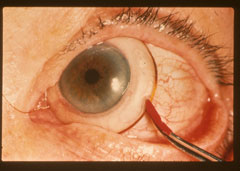
\includegraphics[width=0.35\textwidth]{cap_02_et_ssg}
					\caption[Ejemplo de uso de SSG]{Ejemplo de uso de SSG\footnotemark.}
					\label{fig:02_et_ssc}
				\end{figure}
				\footnotetext{Fuente imagen: \url{http://www.dizziness-and-balance.com/practice/default.htm}}

				\item \textbf{Electro-OculoGrafía (\acrshort{eog}):} Este método de seguimiento ocular permite determinar la dirección en la que se encuentra direccionado el ojo en base a la medición de diferencias de potencial eléctrico en la piel. En la medida que el ojo rota, el dipolo producido por la córnea y la retina cambia su orientación, lo que se ve reflejado en los potenciales de las zonas aledañas. Sus ventajas principales, además del bajo costo, son la capacidad de medir el movimiento ocular incluso aunque los ojos se encuentren cerrados (lo que hace de este método una herramienta interesante en casos de estudio de sueño) y que las mediciones son relativas a la posición de la cabeza. No obstante lo anterior, la precisión y exactitud de las mediciones obtenidas es baja ya que se encuentran sujetas a artefactos como el movimiento de los párpados. La figura \ref{fig:02_et_eog} muestra el posicionamiento típico de los electrodos en este tipo de \textit{\gls{setup}}. 
				\begin{figure}[H]
					\centering
					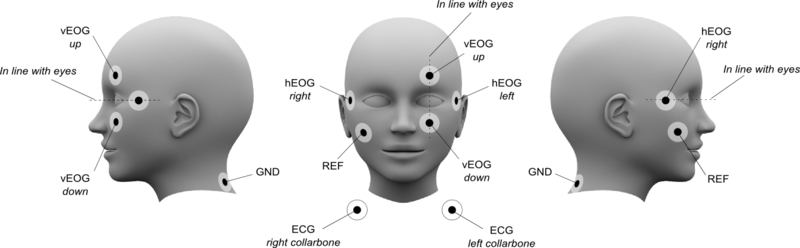
\includegraphics[width=0.9\textwidth]{cap_02_et_eog}
					\caption[Ejemplo de posicionamiento de electrodos para EOG]{Ejemplo de posicionamiento de electrodos para EOG\footnotemark.}
					\label{fig:02_et_eog}
				\end{figure}
				\footnotetext{Fuente imagen: \url{http://sbiwiki.cns.ki.se/mediawiki/index.php/Natmeg/checklist_MEG_preparation}}

				\item \textbf{Seguimiento ocular basado en video (\acrshort{vog}):} Este método de seguimiento ocular es el más popular en la actualidad. Consiste en capturar, con una o más cámaras, la actividad ocular y mediante procesamiento de imágenes determinar en que dirección se encuentra orientada la mirada. El procesamiento puede ser dividido en dos etapas principales: en la primera se detecta y localiza el ojo en la imagen, para lo que típicamente se utiliza la pupila o el iris y la segunda etapa corresponde al proceso por el cual se estima hacia donde se encuentra dirigido. 

				Dentro de las técnicas VOG existentes la más utilizada corresponde a la estimación mediante reflexión corneal (con una fuente de luz típicamente infrarroja (\acrshort{ir})) y detección de pupila. Los focos de luz se ubican de forma que siempre se encuentren en la misma posición respecto del ojo, con lo cual la reflexión se mantiene virtualmente siempre en el mismo lugar. De esta forma la estimación se genera en base a la diferencia entre la ubicación de centro de la pupila y la posición de la reflexión.  

				El principio de funcionamiento asociado a este método se basa en las imagenes de Purkinje-Sanson que describen la existencia de al menos 4 reflexiones de luz producidas por la córnea y el cristalino (figura \ref{fig:02_et_vog1} (a)) que pueden ser utilizadas como referencia para estimar el direccionamiento del ojo. En la figura \ref{fig:02_et_vog1} (b) es posible observar la primera reflexión de Purkinje en relación a distintas posiciones de la pupila.
				\begin{figure}[H]
					\centering
					\subfloat[Reflexiones de Purkinje-Sanson]{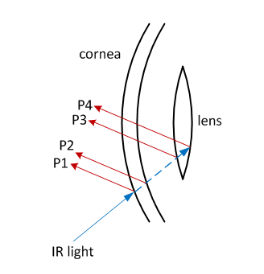
\includegraphics[width=0.3\textwidth]{cap_02_et_vog1}}\hspace{5mm}
					\subfloat[Posición de la reflexión P1 relativa al centro de la pupila.]{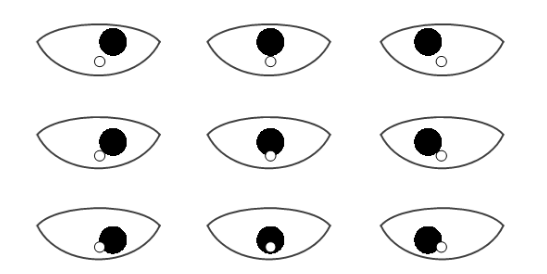
\includegraphics[width=0.55\textwidth]{cap_02_et_vog2}}
					\caption[Principio de detección VOG en base a reflexión de luz]{Principio de detección VOG en base a reflexión de luz\cite{dissertation:eyetrackers}.}
					\label{fig:02_et_vog1}
				\end{figure}

				La presentación de estos dispositivos es variada y van desde cascos y lentes hasta trípodes y columnas donde se integran un elemento apoya-baribilla y el \textit{eye tracker}, como en la figura \ref{fig:02_ejemplo_setup}. En la figura \ref{fig:02_et_vog2} se muestra un par a modo de referencia. 
				\begin{figure}[H]
					\centering
					\subfloat[Tobii Pro Glasses 2]{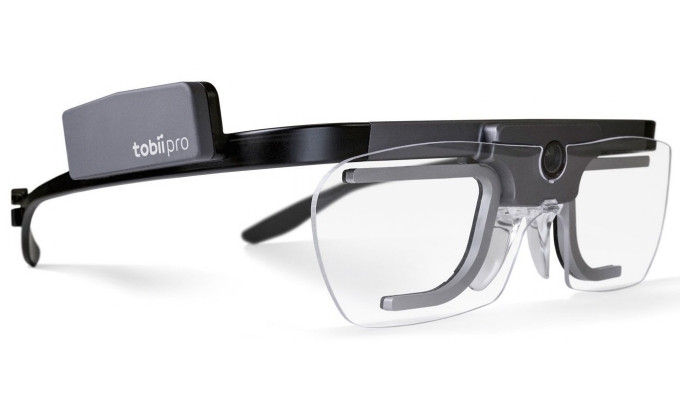
\includegraphics[width=0.4\textwidth]{cap_02_et_vog_1}}\hspace{5mm}
					\subfloat[MiraMetrix S2]{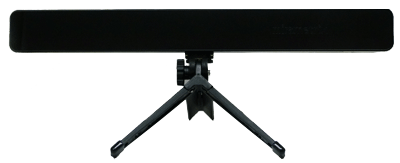
\includegraphics[width=0.4\textwidth]{cap_02_et_vog_2}}
					\caption[Muestra de \textit{eye trackers} disponibles en el mercado con tecnología VOG basados en reflexión de luz \acrshort{ir}]{Muestra de \textit{eye trackers} disponibles en el mercado con tecnología VOG basados en reflexión de luz \acrshort{ir}\footnotemark.}
					\label{fig:02_et_vog2}
				\end{figure}
				\footnotetext{Fuente imagen: \url{https://www.tobii.com/} y \url{https://www.microway.com.au/} respectivamente.}

			\end{enumerate}

		\subsection{Comparacióen entre tecnologías}
		\label{sub:02_comparativa_eyetracker}
			En la literatura consultada \cite{dissertation:eyetrackers, article:eyetracker_eggert, article:eyetracker_richardson} se entregan nociones sobre las capacidades operativas que se resumen en la tabla \ref{tbl:eyetracker_compare} para EOG, SSG, VOG (común) y DPI (VOG de gama alta utilizando distintas reflexiones de Purkinje). 

			En esta, es posible evidenciar a grandes rasgos la cantidad de parámetros a considerar en el proceso de elección de una tecnología particular: Debe existir un compromiso entre la comodidad para el usuario, las prestaciones tanto en precisión temporal como espacial, dificultad para obtener una buena calibración, etc. De forma tal que permitan la ejecución de cierto tipo de experimentos. 

			Si lo que interesa medir corresponde al efecto de, por ejemplo, las micro-sacadas en el proceso visual, la principal preocupación se centra en obtener una alta precisión espacial y temporal con el fin de caracterizar correctamente estos movimientos. Por otro lado, si lo que interesa estudiar son los patrones de comportamiento de usuarios para un estudio de usabilidad\footnote{Estudios enfocados en caracterizar la experiencia de usuario e identificar el comportamiento del mismo en alguna plataforma (pagina web, aplicación, etc.).} en un sitio web, estas variables no son tan importantes como la comodidad del usuario, ya que sus acciones deben corresponder lo más posible a una situación común, con el fin de reflejar correctamente sus intereses.  
			\begin{table}[H]\begin{center}\footnotesize{
				\singlespacing{\begin{tabular}{| C{0.18\textwidth} | C{0.18\textwidth} | C{0.18\textwidth} | C{0.18\textwidth} | C{0.18\textwidth}|}
					\hline
					 & EOG & SSG & VOG & DPI \\ \hline
					Precisión espacial (grados)	& $\approx 0.5$ & $\approx 0.01$ & $\approx 0.05$ & $\approx 0.017$\\ \hline
					Precisión temporal\footnotemark (Hz) 	& $40$ & $500$ & $50-400$ & $500-1000$\\ \hline
					Registro de mov. verticales	& Es posible pero se encuentran sujetos a error por efecto de artefactos producidos por el párpado & Si & Si & Si \\ \hline
					Registro de torsión			& No & Si & Si & Si \\ \hline
					Tiempo de \textit{setup}		& Lento debido a que requiere la utilización de electrodos & Lento & Rápido & Rápido \\ \hline
					Requiere calibración por enfoque & Si & No & Si & Si \\ \hline
					Complejidad de calibración	& Requiere configuración bitemporal & La no-linealidad puede ser compensada con un modelo basado en ajuste de parámetros & Buena linealidad & Buena linealidad \\ \hline
					Invasividad 				& Electrodos cercanos al ojo (sin contacto), no afecta el campo visual & Lentes de contacto, posibles efectos negativos en precisión visual, incomodidad & Aparato montado en la cabeza (sin contacto con los ojos), limitación moderada del campo visual & Cabeza inmovilizada en un soporte de barbilla, limitación moderada del campo visual \\ \hline
				\end{tabular}}
				\caption[Comparativa de los sistemas de adquisición encontrados]{Comparativa de los sistemas de adquisición encontrados en \cite{dissertation:eyetrackers, article:eyetracker_eggert, article:eyetracker_richardson}.}
				\label{tbl:eyetracker_compare}
			}\end{center}\end{table}
			\footnotetext{Frecuencia de muestreo.}	

	% ===============================================================
	% ===============================================================
	\vspace{-10mm}
	\section{Métodos de estimulación visual}
	\label{sec:02_sistemas_de_estimulacion_visual}
		\subsection{Hardware de estimulación}
		\label{sub:02_hardware_de_estimulacion}
			Debido a que la presentación de resultados de investigación científica requieren de que los datos obtenidos sean comprobables y los experimentos reproducidos, es que se hace necesario declarar de forma precisa las características de los estímulos, métodos utilizados para adquirir datos y técnicas aplicadas en el procesamiento posterior. Por lo cual, la elección del artefacto de estimulación es una tarea particularmente sensible \cite{article:monitor_beuer}.

			A lo largo de la historia, los investigadores dedicados al estudio del movimiento ocular han usado diversas tecnologías con el propósito de estimular visualmente a sus pacientes, no obstante, no fue hasta la década de los 70' y de la mano de los computadores, que los monitores \acrshort{crt} revolucionaron este campo de investigación convirtiéndose en el estándar durante décadas. El motivo principal de su popularidad dice relación con la capacidad que brindan, mediante la programación en computador, de diseñar con relativa facilidad una gran gama de pruebas y experimentos distintos, lo que permitió explorar de forma rápida nuevos métodos e hipótesis. Esto, complementado a la integración del control de los parámetros de estimulación y almacenamiento de resultados e historiales en el mismo dispositivo permitió robustecer los procesos de investigación debido a la capacidad de repetir los experimentos sin afectar las características de los estímulos. 

			Las limitantes de los primeros dispositivos se fueron subsanando con el avance de la tecnología, de esta forma, los monitores análogos avanzaron hasta alcanzar tasas de refresco elevadas ($\geq 200[Hz]$), una gran gama de colores, buena resolución espacial (alcanzando hasta $1600[px]$ de ancho), un rápido decaimiento del fósforo de la pantalla que se traduce en tiempos de repuesta reducidos ($< 1[ms]$) y un buen tamaño (típicamente $20[pulg]$ en la diagonal). En base a esta información pueden definirse dos conceptos relevantes para el hardware de estimulación: 
			\begin{enumerate}\setlength\itemsep{-0.2em}
				\item \textbf{Tasa de refresco (\acrshort{fps}):} Dice relación con la cantidad de veces que se actualiza la imagen de la pantalla por cada segundo. Influye en el timing de los estímulos.
				\item \textbf{Tiempo de respuesta (\acrshort{rt}):} Es cuanto demora un pixel de la pantalla en cambiar su color de blanco a negro. Influye en la calidad y nitidez de las imágenes. 
			\end{enumerate}

			A pesar de la mejoras considerables en sus características, las nuevas tecnologías han hecho desaparecer a los monitores CRT del mercado, siendo más comunes ahora monitores LCD, LED y oLED que tienen pantallas de mayor tamaño, menor consumo de energía, menor radiación electromagnética y una menor huella de carbono. Es importante destacar que, a pesar de que el aspecto de las nuevas tecnologías es similar, sus principios de funcionamiento, capacidades y características difieren.

			Existen varias consideraciones que hacer al utilizar estas tecnologías \cite{article:monitor_wang, article:monitor_elze}. Transversalmente se tiene un problema de \textit{timing} debido a las bajas tasas de refresco de la mayor parte de los monitores modernos, lo que vuelve una tarea no trivial el cumplir con los requerimientos de los estímulos y evitar que el usuario perciba una falta de fluidez en la presentación, lo que podría producir que distraiga su atención. En este sentido, por ejemplo, aunque muchos monitores modernos indican que su tasa de refresco se encuentra entre $60-75[Hz]$, no se aclara en sus hojas de datos cual es el límite efectivo. Este punto se vuelve crítico si se considera que una buena parte de los equipos modernos incorporan sistemas de procesamiento de imagenes para mejorar la calidad, lo que retrasa aún mas estos tiempos. 

			Otro elemento de cuidado es el tiempo de respuesta. Si este es elevado, producirá un efecto de halos o rastros de luz cuando las imágenes se mueven con rapidez, por esto, es ideal asergurar que este sea reducido para lograr que el cambio entre imágenes no sea notorio y afecte el experimento (esto se hace más presente en casos en los que se muestra secuencias de video). 

			Finalmente, es importante compaginar las características del experimento con las propiedades lumínicas del equipo ya que es sabido que en tecnologías como la de los monitores LCD tanto el ángulo del observador respecto de la pantalla como las distintas zonas de la misma afectan el color/contraste observado (efecto de retro-iluminación). 
			
		\subsection{Software de estimulación}
		\label{sub:02_software_de_estimulacion}

			Tal como se indicó en el apartado anterior la generación de estímulos es una pieza clave en la realización de experimentos ya que permiten preparar un escenario adhoc para la obtención de datos específicos. En el sitio web de Hans Strasburger \cite{website:software} es posible encontrar una larga lista de software especializado para el desarrollo de experimentos en el área de la psicofísica además de referencias e información sobre sus características. A modo de resumen se presenta en el cuadro \ref{tbl:systems_compare} una comparación entre algunas de las aplicaciones indicadas en la página\footnote{Esta selección fue realizada en base al número de citas para cada aplicación en Google Scholar.}.  
			\begin{table}[H]\begin{center}\footnotesize{
					\singlespacing{\begin{tabular}{| C{0.2\textwidth} | C{0.16\textwidth} | C{0.16\textwidth} | C{0.16\textwidth} | C{0.16\textwidth} |}
					\hline
					 								& PsychoPy 	& VissionEgg & PsychoToolbox & Stimulus Presentation \\\hline
					Tipo de software 				& \multicolumn{3}{c|}{Open source} & Privativo, de pago \\\hline
					Plataforma 						& \multicolumn{2}{c|}{python + OpenGL} & Matlab/Octave & Software independiente (IDE con editor de python) \\\hline
					Sistema operativo 				& \multicolumn{3}{c|}{Linux, MacOS, Windows} & Windows \\\hline
					Fecha de última actualización 	& $Dec/2017$ & $Sep/2014$ & $Oct/2017$ &  $Abr/2017$ \\\hline
					Citaciones en Google Scholar 	& $2220$ 	& $427$ 	& $6310$ 	& $3520$\\\hline
					Programable 					& \multicolumn{4}{c|}{Si}\\\hline
					Imágenes y Video 				& \multicolumn{4}{c|}{Si}\\\hline
					Sonido 							& \multicolumn{4}{c|}{Si}\\\hline
					Soporte para \textit{Eye trackers} incluido 	& Si 		& No 		& Si 		& Si\\\hline
					Capacidad para registro de data 	& Si 		& No 		& Si 		& Si\\\hline
					Documentación/Foro disponible 			& Si 		& No (Link caído) & Si 	& Si\\\hline
				\end{tabular}}
				\caption[Comparativa de software de estimulación]{Comparativa de software de estimulación \cite{website:software_presentation, website:software_psychopy, website:software_psychotoolbox, website:software_vissionegg}.}
				\label{tbl:systems_compare}
			}\end{center}\end{table}

		\vspace{-10mm}
		\subsection{Experimentos de estimulación}
		\label{sub:02_experimentos_de_estimulacion}
			Debido a la versatilidad de los movimientos sacádicos, se ha desarrollado con el tiempo un número importante de tareas sicomotoras para probar distintos mecanísmos cognitivos. Por este motivo y a modo de acotar las actividades asociadas a este trabajo de título, se desarrollará el sistema propuesto de forma tal que permita solo la implementación de experimentos con características similares a los presentados en \cite{article:tests_1, article:tests_2, article:tests_3, article:tests_4, article:tests_5}, que corresponden a métodos utilizados en la evaluación y caracterización de desempeño sicomotor en pacientes que padecen la enfermedad de Parkinson. Dichas tareas corresponden a la evaluación de movimientos pro-sacádicos, anti-sacádicos y aquellos guiados por memoria.

			En la explicación de estos experimentos se utilizarán dos elementos importantes. El primero corresponde al punto de fijación o \acrshort{fp} y el segundo al punto objetivo o \acrshort{tp}. FP es un punto ubicado en el centro de la estimulación a modo de referencia y se utiliza para calcular las amplitudes de los movimientos oculares. TP es un punto objetivo que sirve como guía en la realización de los movimientos. 

			\vspace{-5mm}
			\subsubsection{Métricas de interés}
			\label{ssub:metricas_de_interes}
				Las métricas principales a considerar para este tipo de experimentos son:
				\begin{enumerate}\setlength\itemsep{-0.2em}
				 	\item \textbf{Latencia sacádica (\acrshort{sl}):} Lapso de tiempo que transcurre entre la aparición de un nuevo estímulo y el comienzo de una sacada $[ms]$. 

				 	\item \textbf{Intervalo inter-sacádico (\acrshort{isi}):} Tiempo entre el término de un movimiento sacádico y el comienzo de otro en $[ms]$.
				 	
				 	\item \textbf{Ganancia inicial de movimiento:} Cociente entre la amplitud de la sacada y la distancia desde el punto de partida al objetivo. 
				 	
				 	\item \textbf{Tasa de error:} Relación entre el número de veces que el movimiento ejecutado fue errado y el total de movimientos realizados. 

				 \end{enumerate} 

			\vspace{-5mm}
			\subsubsection{Movimientos pro/anti sacádicos}
			\label{ssub:movimientos_pro_anti_sacadicos}
				Aunque se parecen en estructura, el enfoque de estas tareas es completamente distinto. La medición de la respuesta prosacádica tiene como fin el cuantificar la capacidad del individuo para responder de forma reflexiva frente a un nuevo objetivo y entrega información que suele utilizarse como base para comparar otros métodos. Por otro lado, la actividad antisacádica implica la inhibición del comportamiento reflexivo y la realización de un movimiento voluntario en la dirección opuesta, de esta forma la información obtenida permite conocer el estado de estructuras cerebrales como el lóbulo frontal, en donde se procesan las funciones ejecutivas.	
				\begin{figure}[H]
					\centering
					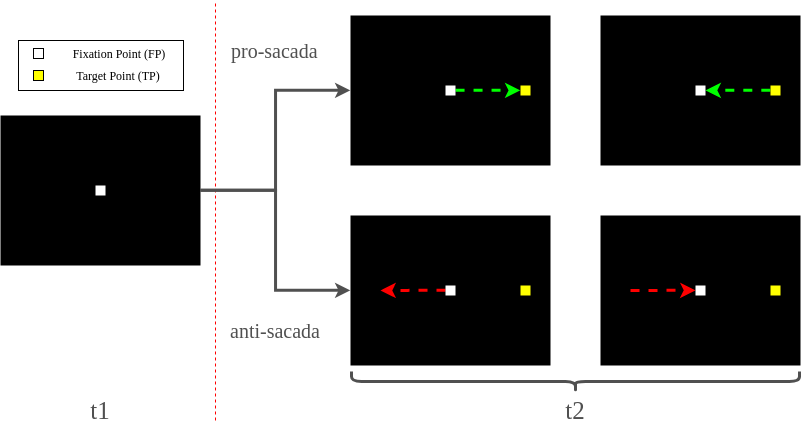
\includegraphics[width=0.8\textwidth]{cap_02_proantisaccade_base}
					\caption{Tarea pro/anti sacádica.}
					\label{fig:02_pro_anti_saccade_base}
				\end{figure}  

				Los tipos de movimientos descritos se estudian mediante estímulo similares al propuesto en la figura \ref{fig:02_pro_anti_saccade_base}. Usualmente se pide al sujeto que mantenga su vista en $FP$ (blanco) durante algún tiempo $t_1$ hasta que aparezca $TP$ (amarillo) y luego realice la tarea solicitada, para lo cual se otorga un tiempo $t_2$. En el caso de los movimientos prosacádicos, como ya fue explicado con anterioridad, se debe rotar los ojos hacia $TP$ y luego volver a $FP$ (flechas verdes). Para movimientos antisacádicos se realiza la acción contraria (flechas rojas). En algunos casos resulta conveniente añadir una imagen de feedback al final del experimento para indicar si la tarea fue realizada correctamente. 

				Estos experimentos pueden ser modificados y complementados con el fin de estudiar actividades cognitivas más complejas. Típicamente estas variaciones aplican uno o más paradigmas como los que se muestran en la figura \ref{fig:02_paradigmas}, donde puede apreciarse un diagrama de temporización de un estímulo bajo el efecto de los paradigmas de gap, overlap y delay. 
				\begin{figure}[H]
					\centering
					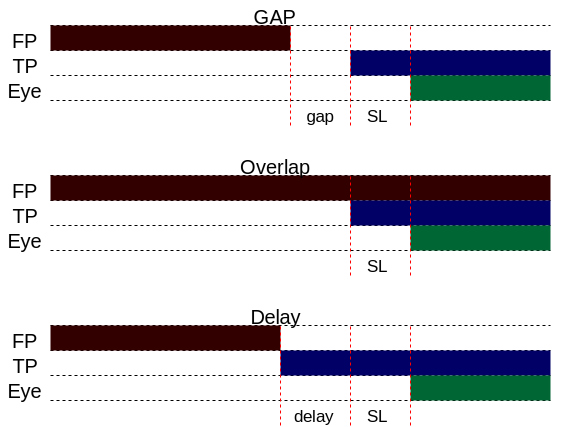
\includegraphics[width=0.5\textwidth]{cap_02_paradigmas}
					\caption{Paradigmas de experimentación.}
					\label{fig:02_paradigmas}
				\end{figure} 

				Donde $FP$ es el Fixation Point, $TP$ el Target Point, $Eye$ representa si existe o no movimiento ocular (o más bien, cuando se espera que ocurra) y $SL$ corresponde a la latencia sacádica.  

			\vspace{-5mm}
			\subsubsection{Movimientos guiados por memoria}
			\label{ssub:movimientos_memoria}
				Los experimentos guiados por memoria corresponden a tareas en las cuales el usuario debe repetir con movimientos oculares algun patrón observado con anterioridad. 

				En la figura \ref{fig:02_memory} es posible observar un diseño simple para este tipo de experimentos. Despues de mantener $FP$ por un lapso $t_1$ en pantalla se muestra una serie de objetivos $T_n$ en intervalos de tiempo idénticos, luego se muestra nuevamente $TP$ por un lapso $t_3$ para indicar que ha finalizado la serie y dar tiempo al usuario para prepararse. Finalmente se solicita que se muevan los ojos en secuencia por los puntos en que se vio aparecer los objetivos.
				\begin{figure}[H]
					\centering
					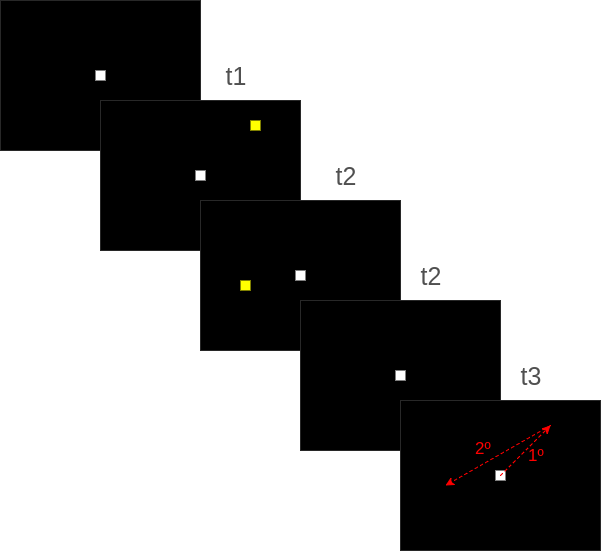
\includegraphics[width=0.65\textwidth]{cap_02_memory}
					\caption{Tarea guiada por memoria.}
					\label{fig:02_memory}
				\end{figure} 
	
	% ===============================================================
	% ===============================================================
	\section{Sistemas de estimulación y registro visual}
	\label{sec:02_sistemas_de_estimulacion_registro_visual}
		A continuación se muestran los elementos principales requeridos para la configuración y puesta en marcha de un sistema de estimulación visual y registro de movimiento ocular según lo propuesto por Scott MacKenzie en \cite{article:baseInfo}. 

		En la figura \ref{fig:02_ejemplo_setup} se presenta a modo de ejemplo un \textit{setup} típico en estudios de movimiento ocular. Su configuracón consiste en un monitor LCD, un \textit{eye tracker} de trípode que en este caso se encuentra montado en un apoya-barbilla y un teclado en el caso de requerir interacción con el usuario. El apoya-barbilla cumple dos funciones sumamente importantes: Mantiene al usuario a una distancia determinada de la pantalla, lo que permite generar estímulos en un rango visual específico y ayuda al paciente a no mover su cabeza durante el experimento, con lo cual se evitan distorsiones en las mediciones realizadas por el \textit{eye tracker}.  

		\begin{figure}[H]
			\centering
			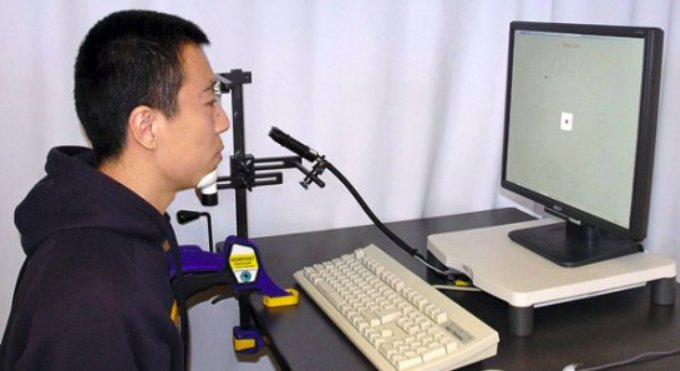
\includegraphics[width=0.5\textwidth]{cap_02_setup}
			\caption[\textit{Setup} experimental típico]{\textit{Setup} experimental típico \cite{article:baseInfo}.}
			\label{fig:02_ejemplo_setup}
		\end{figure}

		En la figura \ref{fig:02_diagrama_interfaz} se pretende explicitar la función del sistema de estimulación - adquisición - registro y los requerimientos del mismo. El software asociado al sistema debe ser capaz de manejar la interfaz con el usuario para poder entregar estímulos (visuales principalmente) y recibir las respuestas asociadas (en forma de datos de posicionamiento ocular o respuestas solicitadas por pantalla) de forma de agrupar las acciones temporalmente, permitiendo de esta forma dar sentido a los datos obtenidos en el experimento. 
		
		\begin{figure}[H]
			\centering
			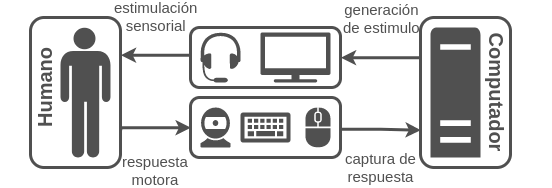
\includegraphics[width=0.7\textwidth]{cap_02_diagram}
			\caption[Diagrama general de la interfaz hombre-máquina]{Diagrama general de la interfaz hombre-máquina \cite{article:baseInfo}.}
			\label{fig:02_diagrama_interfaz}
		\end{figure}

	% ===============================================================
	% ===============================================================
\end{document}
